\documentclass{standalone}
\usepackage{pgfplots}
\usepackage{amsmath}
\usepackage{cite}

\begin{document}

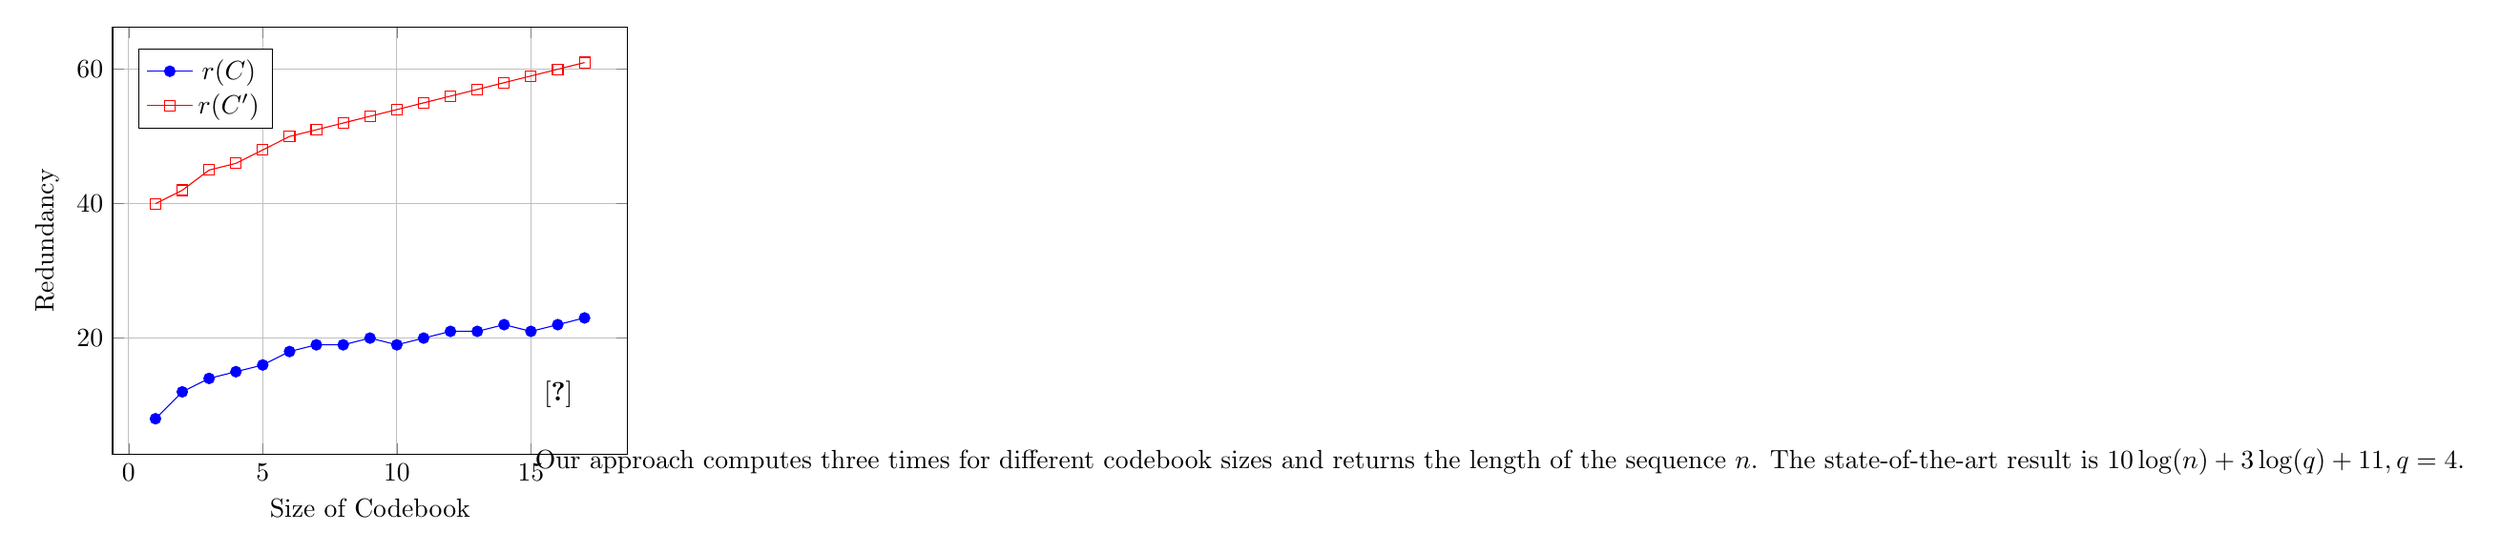
\begin{tikzpicture}
    \begin{axis}[
        xlabel={Size of Codebook},
        ylabel={Redundancy},
        legend style={at={(0.05,0.95)}, anchor=north west},
        grid=major,
    ]
    
    % Plot for r(C)
    \addplot[
        color=blue,
        mark=*,
        ]
        coordinates {
            (1, 8)
            (2, 12)
            (3, 14)
            (4, 15)
            (5, 16)
            (6, 18)
            (7, 19)
            (8, 19)
            (9, 20)
            (10, 19)
            (11, 20)
            (12, 21)
            (13, 21)
            (14, 22)
            (15, 21)
            (16, 22)
            (17, 23)
        };
    \addlegendentry{$r(C)$}
    
    % Plot for r(C')
    \addplot[
        color=red,
        mark=square,
        ]
        coordinates {
            (1, 40)
            (2, 42)
            (3, 45)
            (4, 46)
            (5, 48)
            (6, 50)
            (7, 51)
            (8, 52)
            (9, 53)
            (10, 54)
            (11, 55)
            (12, 56)
            (13, 57)
            (14, 58)
            (15, 59)
            (16, 60)
            (17, 61)
        };
    \addlegendentry{$r(C')$}
    
    \end{axis}
    
    \node at (5.5,0.5) [anchor=south west] {\cite{Smagloy_Welter_Wachter-Zeh_Yaakobi_2020}}; % Citation near the plot
    \node at (5.5,0.2) [anchor=north west] 
    {Our approach computes three times for different codebook sizes and returns the length of the sequence $n$. The state-of-the-art result is $10 \log(n) + 3 \log(q) + 11, q=4$.};
    
\end{tikzpicture}

\end{document}